\documentclass[tikz,border=4pt]{standalone}
\usepackage{amsmath}
\usepackage{tikz}
\usetikzlibrary{arrows.meta,calc,decorations.markings}

\begin{document}
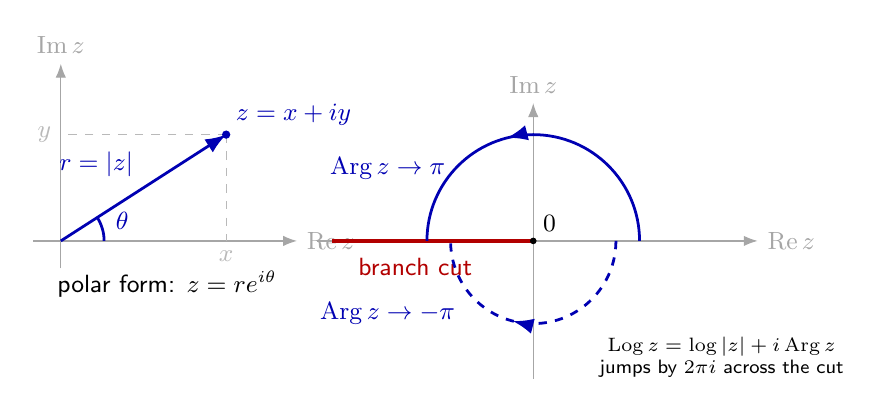
\begin{tikzpicture}[
  >=Latex,
  axis/.style={gray!70,->,line width=0.45pt},
  cut/.style={red!70!black,line width=1.2pt},
  ray/.style={blue!70!black,line width=1pt},
  note/.style={font=\small\sffamily}
]
  \begin{scope}
    \draw[axis] (-0.35,0) -- (3.0,0) node[right,note] {$\operatorname{Re}z$};
    \draw[axis] (0,-0.35) -- (0,2.25) node[above,note] {$\operatorname{Im}z$};
    \coordinate (O) at (0,0);
    \coordinate (Z) at (2.1,1.35);
    \draw[dashed,gray!55] (Z) -- (2.1,0) node[below,note] {$x$};
    \draw[dashed,gray!55] (Z) -- (0,1.35) node[left,note] {$y$};
    \draw[ray,->] (O) -- (Z) node[midway,above left,note] {$r=|z|$};
    \fill[blue!70!black] (Z) circle (1.5pt) node[above right,note] {$z=x+iy$};
    \draw[ray] (0.55,0) arc[start angle=0,end angle=32.7,radius=0.55];
    \node[note,blue!70!black] at (0.78,0.25) {$\theta$};
    \node[note] at (1.35,-0.55) {polar form: $z=re^{i\theta}$};
  \end{scope}

  \begin{scope}[xshift=6.0cm]
    \draw[axis] (-2.75,0) -- (2.85,0) node[right,note] {$\operatorname{Re}z$};
    \draw[axis] (0,-1.75) -- (0,1.75) node[above,note] {$\operatorname{Im}z$};
    \draw[cut] (-2.55,0) -- (0,0);
    \node[note,red!70!black,below] at (-1.5,-0.1) {branch cut};
    \draw[ray,postaction={decorate},
      decoration={markings,mark=at position 0.58 with {\arrow{Latex}}}]
      (1.35,0) arc[start angle=0,end angle=180,radius=1.35];
    \draw[ray,dashed,postaction={decorate},
      decoration={markings,mark=at position 0.58 with {\arrow{Latex}}}]
      (1.05,0) arc[start angle=0,end angle=-180,radius=1.05];
    \node[note,blue!70!black] at (-1.85,0.92) {$\operatorname{Arg}z\to\pi$};
    \node[note,blue!70!black] at (-1.85,-0.92) {$\operatorname{Arg}z\to-\pi$};
    \node[font=\scriptsize\sffamily,align=center,anchor=west] at (0.72,-1.48)
      {$\operatorname{Log}z=\log|z|+i\operatorname{Arg}z$\\ jumps by $2\pi i$ across the cut};
    \fill[black] (0,0) circle (1.2pt) node[above right,note] {$0$};
  \end{scope}
\end{tikzpicture}
\end{document}
